\chapter{Literature Review}
\label{chap:literature_review}

% focused, concise
% supports the well-stated question
% identifies a gap
% reports and critiques current state of discourse
% critical
% adds value

% motivation

Given the aims identified in the introduction, this chapter investigates the existing work that can help us understand the \emph{framing} phenomenon, and how it has been detected by automatic approaches, usually performed on single articles.
% how we can expand the current state of detection by using the information coming from other articles.
But, as mentioned previously, this type of analysis struggles to detect the framing when it is very subtle and manifests through techniques such as focusing on certain aspects, or selecting which details to include or omit, or even selecting a specific order inside a story~\cite{morstatter2018identifying}.
For these specific cases, it is very complicated to spot what belongs to framing or not, and we argue that an automated analysis would benefit from comparing different articles that talk about the same event but have different perspectives. %taking a look at other articles.

This multi-article knowledge requires introducing a second family of methods that aims at finding \emph{similarities} between articles, by using document and sentence representations, and to find which pieces appear in multiple documents. In this way the common ground can be identified, as well as the diversity in the information reported.
With this second family of methods we can see that for a certain event there are several articles which overlap in part, and some have unique pieces or specific words that differ from the others. But this analysis needs an interpretation framework that is able to describe the framing role of the choices done by each of the sources.

Exploring these two different fields of research, we can see that there is an intersection area that is not much explored, that is the analysis of framing differences. Given the differences identified by this second group of methods, we need to expand the framing analysis to work with multiple documents and understand why modifications in the text happen.
We have some works that analyse this specific field, but using manual handcrafted analysis, that for example show how events are described from sources belonging to different political leanings. We want to target this specific area with an automated analysis.
%under the perspective of social science (manual analysis, not automated), and the automation of this type of analysis is an existing gap.

% structure

For these reasons, this chapter is structured in three parts: framing analysis of single documents (Section~\ref{sec:lit_framing}), similarities between multiple documents (Section~\ref{sec:lit_relationships}) and finally the point of contact between the two (Section~\ref{sec:lit_gap}), as our target niche.

% The structure of 2.1 and 2.2 is inside 2.1 and 2.2
% expanding on framing theories in Section~\ref{ssec:lit_framing_theory}, then moving to automated framing analysis in Section~\ref{ssec:lit_framing_auto}. Section~\ref{ssec:lit_framing_other} is providing some insights about related analyses that are quite related to framing (e.g., subjectivity, source bias and factuality) and Section~\ref{ssec:lit_framing_limit} exposes the limits of the single-article framing analysis.
% Then we move to the second area, that is ~\ref{sec:lit_relationships}: 
% We are considering two main research areas that are related to our problem: \textit{i)} framing analysis and \textit{ii)} analysis of similarities between documents.

\section{Framing}
\label{sec:lit_framing}

% definition
As we are using the term \emph{framing}, we need to define what we mean with it, because multiple definitions do exist.
% Before exploring the framing analysis area, we need to define what we mean with framing, because multiple definitions exist.
% - broad framing as perception of the world (goffman)
The broadest definition comes from \citet{goffman1974frame} who defines framing as how people organise experiences about the world.
% - semantic frames
Then we have the Frame Semantics~\cite{fillmore2006frame} that instead defines a frame as ``\textit{any system of concepts related in such a way that to understand any one of them you have to understand the whole structure in which it fits}''. This second definition goes into the direction of annotating sentences with units of meaning (semantics) that are evoked by specific words, e.g. FrameNet~\cite{baker1998berkeley}.

% - media framing
But the definition that we rely on, instead focuses on the power of media to present facts under a specific light: instead of focusing on \emph{what} is contained in a text (semantics), we focus on \emph{how} it is described.
This facet of the term \emph{framing} can be seen in the work of
\citet{entman1993framing} that defines framing as ``\textit{select[ing] some aspects of a perceived reality and make them more salient in a communicating text}''.
Or from \citet{goffman1974frame} that describes framing as ``\textit{how a certain story is presented to shape mass opinion}''.
% some description and insight about how it is described
Using this connotation, framing becomes an additional layer on top of the factual information focusing on the presentation side, giving a structure (identifying problems, causes, resolutions) where each of the semantic elements is given a role to create a coherent story~\cite{pan1993framing}.



% ``the central organising themes ... that connect different semantic elements of a news story (headlines, quotes, leads, visual representations, and narrative structure) into a coherent whole to suggest what is an issue.''~\cite{pan1993framing}

% Structure of 2.1
We expand in the following on \textit{i)} framing theories, where we can see which techniques have been defined in previous research, then we move to practical framing detection models and finally to the identification of concepts that are very much related to framing but have an independent meaning.
% We are expanding on framing theories in Subection~\ref{ssec:lit_framing_theory}, then moving to automated framing analysis in Subection~\ref{ssec:lit_framing_auto}. Subection~\ref{ssec:lit_framing_other} is providing some insights about related analyses that are quite related to framing (e.g., subjectivity, source bias and factuality) and Subection~\ref{ssec:lit_framing_limit} exposes the limits of the single-article framing analysis.

\subsection{Framing theories and definitions}
\label{ssec:lit_framing_theory}
% framing: definition and theory

% We have a group of theoretical studies that define the concept of \textit{media framing}~\cite{gamson1989media,scheufele2007framing},

% concepts
Media framing, under the theoretical side, is composed of several concepts and processes~\cite{scheufele1999framing}.
% 1. frame building
\textit{Frame building} is the process of creating a narrative in which the articles can fit. It corresponds to defining the objectives of the communication in which several articles can be fitted document coherent to them.
%~\cite{scheufele1999framing}
It produces ``media frames'' that are embedded in the articles.
% 2. frame setting
Then there is the process of \textit{frame setting} that refers to transferring the frame from the writer to the consumer. How the document has been written creates the ``audience frames'': the reader is placed in a certain mental perspective. For this to happen, a big role is played by the selection of media coverage (which issues to cover or not, with what emphasis, how to fit them into a broader coherent narrative that has been built).
% % 3. individual level effects of framing
% And then there is the individual effects on the audience, in other words the internalisation (attribution of responsibilities, attitudes, behaviours).

Another term that is quite common is ``agenda setting''~\cite{mccombs1972agenda} that corresponds to select the information for the reader (what to think about, not how) that is used to influence the relevance of a certain event: the number of article that are published about each event is an indicator of this process (avalanche effect, a lot of outlets want to have their piece on the same event too).
But the agenda setting ca be seen also at a more fine-grained level: stories are made of details and different sources can emphasise them with different weights.

% and how it acts as an intermediary between the writers and the consumers of the news, via the processes of frame setting and individual-level effects on the public~\cite{scheufele1999framing} (diagram of media vs public and processes)

% Switching from abstract concepts and processes to more tangible, 
Framing is usually defined at macro and micro levels.
For the macro-level, usually, each article is associated with a set of media framing packages, which correspond to a central idea with a surrounding interpretive structure that gives meaning to an issue~\cite{gamson1989media}. And then the micro-level analysis focuses on seeing how the defined frames come out from specific words, used as \textit{framing devices} (e.g., word choice, metaphors, catchphrases, use of contrast, quantification) and \textit{reasoning devices} (e.g., problem definition, cause, consequence, solution, action).

We can take from the literature the following phenomena:

\begin{itemize}
    \item narrative lines / themes (frame building theory, themes, also with stance)
    \item which stories in the coverage (agenda setting)
    \item which details to emphasise (loaded language, headline alignment)
    \item omissions or inclusions (extreme emphasis)
    \item reasoning devices (structural role), problem definition-...  Entman 1993 (as seen in https://www.aclweb.org/anthology/N15-1171.pdf)
    \item subjective language, interpretations and comments
    \item framing packages (metaphors, ....)
    \item loaded language?
\end{itemize}
\todo{reorganise comprehensive list of framing techniques}

% lift RQ1.1: signals
Observing these techniques, we see that all the framing techniques defined in the literature
\todo{motivation for RQ1.1: single-article framing is well defined, but is not enough. Need to extend it}

\subsection{Framing detection}
\label{ssec:lit_framing_auto}
% framing: practical automated approaches

% what is framing detection?
Automated framing detection has been addressed as a task where the objective is to annotate specific pieces of text with labels that express some forms of perspective.

TODO expand

% The approaches used in practice usually come from specifically built lexicons~\cite{TODO} or by human annotations~\cite{card2015media,morstatter2018identifying}.

What framing detection means in literature:
- frames as themes inside an article (e.g. health, energy, security, economy) https://pdfs.semanticscholar.org/f5c8/dbeea0112227486b7fc3bd20a73726ffea88.pdf this corresponds to measuring agenda-setting / attention allocation
- frames as headline point of view (e.g. on articles about gun violence, there can be: gun control vs 2nd amendment vs mental health) https://www.aclweb.org/anthology/K19-1047.pdf + dataset
https://derrywijaya.github.io/GVFC.html
- framing bias: select and emphasize certain facts and interpretations over others when telling their story. Goal: identify type and polarity of framing bias in a sentence: there are 10 defined frames for the selected topic and the classifiers tells which one with the polarity https://isi.edu/~fredmors/paperpdfs/a5-morstatter.pdf
- problem definition, relationship with other problems, people linked, suggested remedy: Entman 1993 (as seen in https://www.aclweb.org/anthology/N15-1171.pdf)
- detection of framing packages  \textit{A frame consists of a variety of components, including “keywords, stock phrases, stereotype images, sources of information” (Entman, 1993, p. 52), “metaphors, exemplars, catchphrases, depictions, [...] visual images” (Gamson and Modigliani, 1989, p. 3), and other devices that provide an interpretive lens or “package.”} https://www.aclweb.org/anthology/N15-1171.pdf
- problem definition, causal interpretation, moral evaluation, and/or treatment recommendation (same as Entman definition) https://onlinelibrary.wiley.com/doi/10.1111/j.1460-2466.2008.00384.x
- Boydstun et al. (2013) suggest that approaches based on hierarchical topic modeling may be an effective means of identifying both issue-specific and generic frames
- what language is perceived as being most related to framing (stereotypes, metaphors, images, catchphrases, and other elements): https://www.aclweb.org/anthology/N15-1171.pdf
- framing and epistemological bias: https://www.aclweb.org/anthology/P13-1162.pdf framing bias is realized by subjective words or phrases linked with a particular point of view. Epistemological bias, is related to linguistic features that subtly (often via presupposition) focus on the believability of a proposition
- quoting patterns as systematic bias https://cs.stanford.edu/people/jure/pubs/quotus-www15.pdf: which new quotes an outlet will select to broadcast. Also tool http://snap.stanford.edu/quotus/vis/
- implicit sentiment / perspective / packaging https://pdfs.semanticscholar.org/3a81/77dc1b3d7aa4948f6cab50a1d3545e476617.pdf
- “entailment,” “implicature,” and “subjectivity” help in identifying framing bias https://www.aclweb.org/anthology/N15-1171.pdf


% resources/datasets
\cite{card2015media} dataset where each document has spans annotated with media frames (broad, non dependent on the specific topic): Economic, Capacity and resources, Morality, Fairness and equality, Legality, constitutionality and jurisprudence, Policy prescription and evaluation, Crime and punishment, Security and defense, Health and safety, Quality of life, Cultural identity, Public opinion, Political, External regulation and reputation, Other.

\cite{morstatter2018identifying} where each sentence has an annotation belonging to specific frames in relationship to the narrow topic of "ballistic missile defense system in Europe": General Threat (GT), Specific Threat (ST), Collective Security (CS), Deterrence System (DS), Domestic Benefit (DB), Progress/Effectiveness (PE), Political Tensions (PT), Threat to Russia (TR), Russian Roadblocks (RR), Partnership with Russia (PR)


% Framing and Linguistic frames (both on a single doc and on multiple docs, e.g. https://journals-sagepub-com.libezproxy.open.ac.uk/doi/pdf/10.1177/1077699015606670)


% On the other hand, there is much literature on \emph{framing}, defined
% as how a certain story is presented to shape mass opinion~\cite{goffman1974frame}, the addition to the underlying facts that reflects the sociocultural context
% %(cultural, political, ...)
% and acts as an underlying force to persuade the reader.
% % Semantic frames~\cite{fillmore2006frame}
% % News Media Frames~\cite{boydstun2014tracking} developed a schema of 15 cross-cutting framing dimensions, such as economics, morality, and politics, and
% % dataset of human annotations~\cite{card2015media}
% The work by~\cite{gamson1989media} describes a set of \emph{framing packages}, made of \emph{framing devices} (e.g., word choice, metaphors, catchphrases, 
% %exemplars, depictions, descriptions, 
% use of contrast, quantification) and \emph{reasoning devices} (e.g., problem definition, cause, consequence, solution, action%, moral evaluation
% ).

\todo{motivation for RQ1.2: framing detection is only done at single-article}


\subsection{Related concepts}
\label{ssec:lit_framing_other}
% framing: exchange with other dimensions

Difference between framing and others:
``framing differs from subjectivity, sentiment, bias, and related constructs. Subjectivity detection may not effectively identify well-established,
codified frames.
Sentiment analysis focuses on assessing the valence
(e.g., positive, neutral, or negative) of an entity’s description. Bias involves a clear, often intentional,
preference shown in writing for one position or opinion on an issue. In contrast, there does not exist
a one-to-one mapping between framing and opinions (Gamson and Modigliani, 1989)
different framings are used to support the same position on an issue. [...] identifying framing requires features and techniques that
go beyond any one of these related concepts.''~\cite{TODO https://www.aclweb.org/anthology/N15-1171.pdf}
Some related concepts:
- hedging: Choi et al. (2012) identify hedging in discussion of GMOs using an SVM trained on n-grams from annotated cue phrases
- sentiment: Greene and Resnik (2009) showed how examining grammatical construction (i.e., syntax) can reveal implicit sentiment;
- bias: Recasens et al. (2013) used edits from Wikipedia intended to enforce a neutral point of view to identify biased sentences and the terms indicative of that bias


\cite{mandal2017overview,gao2018neural,asghar2016automatic} (catchphrases, methaphors, causality).

Framing manifests also through the usage of loaded language, and for this reason, \textit{sentiment and subjectivity analysis} can provide further signals~\cite{liu2010sentiment}.
Sentiment analysis for detecting not only biased news but also comments made by news readers~\cite{park2011politics}.


In addition to these characterisations, we can add other signals derived from studies on \emph{subjectivity}.
% and sentiment intensity.
% https://www.niemanlab.org/2019/05/u-s-journalism-really-has-become-more-subjective-and-personal-at-least-some-of-it/ "a blurring of the line between opinion and fact."
As found by recent research, in contemporary journalism the line between opinion and facts is blurring more and more~\cite{blake2019news}. For this reason, having signals of subjectivity on the document and paragraph-level would be very useful~\cite{liu2010sentiment}.
%Furthermore, subjectivity is closely related to sentiment, since sentiment analysis is about finding the value of opinion while subjectivity is about distinguishing if the text is having an opinion or just reporting factual events~\cite{liu2010sentiment}.
In this way, each article and each paragraph can be characterised with an indication of subjectivity.



And there exist also works that analyse the framing of the whole news source by evaluating factors like political alignment, bias, and factuality~\cite{yin2008truth}.

\todo{link to RQ2.1}

% Alignment of the sources
% Micro-level:
% - Words that evoke framing
% - strong sentiment, loaded language, subjectivity

Narrative structural roles
\cite{zahid2019towards}:
some research considers the \emph{structural role} of a sentence in the document (e.g., is it providing some background, the main event, an evaluation).
Different structural roles have been defined in the literature, such as 
%Different works define sets of structural roles: 
news schema~\cite{bell1991language}, which identifies hierarchical categories (e.g., action, reaction, consequence, context, history), narrative structure~\cite{bell2005news} (e.g., abstract, orientation, evaluation, complication, resolution), or linguistic signals~\cite{zahid2019towards,marcu2000theory}. 
%One recent study~\cite{zahid2019towards} proposed linguistic signals to be able to recognise the structural role.
%With such characterisations, we would be able to add to the sentence-level similarity links also their role in the different articles, to understand how their structure differs.
Such signals could be used to identify the differences between similar sentences with regards to their structural roles in the articles. 
% And this is an important feature because time structure and story structure are usually different~\cite{bell2005news}.

\subsection{Limitations}
\label{ssec:lit_framing_limit}

Limitations of single-article framing analysis
- the method can't see what is missing or added or modified
- narrow to one article only
- can't have external confirmation
- does not see different perspectives, it just shows one side labelling as "framing biased" or not. Bias is everywhere





\section{Similarity between articles}
\label{sec:lit_relationships}

% relationships: motivation
Just analysing the framing of single articles alone provides a good set of signals that can be used to understand the framing that is in action, and this is where the current works on framing belong to. But if we take multiple stories, written by authors with different perspectives, we can use the variety of news to our advantage.
% We need the second area because we want to use methods that can tell us how similar or dissimilar are news articles or sub-parts of them.


% Definition of relationship
There are different possible types of relationships between news articles, such as similarity (covering the same information), referencing (one is citing another one), and temporal proximity. They can be performed at the document level (e.g., the whole article is similar to another one) or at the sentence level (e.g., the same sentence is corroborated by a sentence in another article~\cite{bountouridis2018explaining}) or even at the paragraph level.
Since we are interested in finding articles discussing the same information, we focus on similarity relationships.
% Other relationships could add interesting features, such as the order of publication which would help to identify which of the articles might have taken inspiration from the other. For the time being, we focus on studying and understanding the role of similarity.

% Here in this section, we first describe approaches that deal with language representation, then moving to clustering methods and then finally approaches to plagiarism detection and analysis of how the information repeats in multiple documents.
Here in this section, we first explore what we mean with similarity, then we look at how it is used, and how it is computed, concluding with some limitations of this branch of studies.

\subsection{Similarity definition}
% What is similarity?

Similarity is a pretty straightforward concept: it is defined as ``\emph{the fact that people or things look or are the same}''\footnote{\url{https://dictionary.cambridge.org/dictionary/english/similarity}}. In our case, we take the specific \textbf{semantic textual similarity} from the corresponding benchmark \footnote{\url{http://nlpprogress.com/english/semantic\_textual\_similarity.html}} that expresses how two different pieces of text are similar considering their semantics.
% different liinguistic surface
The similarity can match with how similar the corresponding strings of the text are (character-wise similarity) but has also to account for entities, relationships and concepts can be expressed by using different words that share the same meaning.
For example if we consider two synonyms, their semantic similarity needs to be high. 
% also dependent on the context
And another requirement is that the similarity depends on the context of the words~\cite{miller1991contextual}. The same word can have different meanings depending on the sentence it is used in.
TODO example
\todo{from here on, rewrite 2.2}

\subsection{Applications of similarity}
% What is similarity used for?

Similarity is used in many applications that deal with news/documents.

% Clustering
First of all, in Information Retrieval, a common application is document clustering. Given big quantities of articles





Plagiarism and Manipulation detection (diff\&co)

% TODO figure sent-sent similarity
Some methods are able to extract which information appears in multiple documents or is omitted in some others~\cite{bountouridis2018explaining}, being really useful to analyse the selection of details that each article has made.

% why
Once the articles and parts of them are linked in clusters, there are some works that exploit this information to see how much information is shared between them. This is the field of plagiarism detection, or also some other works that compute how much information is corroborated externally or omitted.



Even for recommender systems (user-items recommendations based on similarity)

\subsection{Similarity computation}
% How is similarity computed?

\subsubsection{Language Representation}
Language representation

% why
This group of methods tackles one question: \emph{What is contained in the text?}

% what (details)
Starting with very naive methods,
Bag of words, stopwords

TF-IDF: how relevant and unique words are\cite{jones1972statistical}

Knowledge extraction: Entity Recognition and Linking, triplets extraction. Is it worth?

The switch to distributional Language models:
first, Word embeddings

The era of Language Models~\cite{devlin2018bert,cer2018universal,yang2019xlnet}.
With the recent explosion of Deep Learning representation there emerged many of Language Model tools that can provide document representation, like BERT~\cite{devlin2018bert}, XLnet~\cite{yang2019xlnet}, or even more oriented towards the similarity task: Universal Sentence Encoder~\cite{cer2018universal}.
And all these models can be used directly without the need to train, thanks to pre-trained models that perform already well out-of-the-box.

% strenghts, limitations
Main strength of Language models:
relate articles that talk about the same events, even if they use different linguistic surface, from articles that may use the same subset of words but talk about different events, it is a semantic matching more than a word-based matching. 

It's a shallower semantic model with respect to the ones based on Entity Linking, but it is more resistant to changes in the linguistic surface.

Talk about SentEval\footnote{\url{http://nlpprogress.com/english/semantic_textual_similarity.html}}: benchmark that evaluates the ability of models to score similarity of sentences


% % language representation
% And with the recent advance of language models~\cite{devlin2018bert,cer2018universal,yang2019xlnet}, we have available robust methods to analyse the overlap of different articles and sub-parts of them by using their representation.







Specific similarity functions: euclidean, cosine, ...





\subsubsection{News Clustering}
Clustering

% why
Once documents and sentences are transformed to a representation, we can apply clustering techniques to find similarity relationships both at the article level (to identify articles that talk about the same event) and at the sentence level (to identify parts of article, details, which are similar, in order to be able to relate sub-document parts).

% what (details)
LDA
methods mostly used are Latent Dirichlet Allocation (LDA) or document embedding.
% News aggregators and LDA topic: can provide article-level aggregation
LDA~\cite{blei2003latent} is the most used technique for topic modelling, as it allows the discovery of topics and to group articles accordingly using word distributions.

Cliques

Distance-based

Hierarchical Clustering

% Topic Detection and Tracking steps
% 0. flat clusters: TDT before 2003. Simple LDA clustering methods
% 1. hierarchical topics: TDT 2003 (hierarchy of topic --> event --> story)
% 2. dependencies: 2004 Napallati~\cite{nallapati2004event}. They introduce edges with two possible reasons: causality or only temporal ordering.

% News event structure evolution (keep short)
% Instead in the direction of the structure of news event, we have a succession of works that went more in details than just creating groups / flat clusters generated by LDA.
% First of all \emph{hierarchical} topic modelling~\cite{allan2003flexible} that defined a set of levels (from the broad concept of topic, to the narrow event that belongs to the topic, and then a specific story/anecdote).
% And then moved to study the dependencies between events~\cite{nallapati2004event} with causality and temporal ordering.
% This recently brought to approaches that are able to find the events belonging to a topic and link them creating a Event Evolution Graph~\cite{yang2009discovering,ansah2019graph} that can be visualised to give an idea of the dependency between the events detected.
%\todo[color=yellow]{The removed paragraph was about events hierarchy and dependency}
% ~\cite{ansah2019graph} that is able to generate a visual story timeline summarisation, connecting the main events; Event Maps~\cite{yang2009discovering}
% Or works that focus on the illustrative side and use the extracted story timeline summarisation~\cite{ansah2019graph}.

% Furthermore, \cite{cai2019temporal} also presents event maps (original baseline~\cite{yang2009discovering}). With also importance score on the nodes and edges. The event relationships can be temporal, content dependence and event dependence.



% strengths, limitations


The literature is quite rich in approaches to news clustering~\cite{carpineto2009survey,jones1972statistical} %also andrews2007recent
that can bring together articles talking about the same events.










\subsubsection{Corroboration analysis}
Corroboration analysis

% what (details)
Furthermore, there are works that not only link the articles at a document level, but also investigate in more detail the connections between sentences.
In one recent work~\cite{bountouridis2018explaining}, groups of similar articles are found, then broken down to pieces of information and analysed to find if these details are \emph{corroborated} (occurring in multiple documents) or \emph{omitted} (occurring in other documents of the same group, but not the current one). 
\todo{figure from Bountouridis paper}
%is good for getting relationships between paragraphs and documents. Corroboration and omission
% \begin{added}
We aim to use this idea of applying similarity to both article-level and sentence-level, extending it even to the word-level. By doing so,
not only we might be able to recognise which sentences appear in multiple documents (with different degrees of similarity) but also we would be able to identify the specific words that have been changed.




Citation Networks?

Edit distances?

Time evolution? TODO find stuff

\subsection{Limitations}
\label{ssec:lit_relationships_limitations}
% The main problems of this set of approaches:
% - analysis of what the differences mean is left to the reader

% strengths, limitations
However, this set of approaches is limited to bringing to the attention of the reader the linked information pieces with a measure of similarity, without characterising the differences. The reader would then need to evaluate the differences in the role of the sentence, the framing that it implies and how it compares with other sentences in terms of subjectivity.
Different documents may express the same set of details, but give them a different role (reporting an action, commenting, contextualising, doing a digression, identifying causes and consequences) and use different words that are semantically similar but may imply a different framing perspective.
% For this reason, the next subsection presents a set of narrative linguistic signals that could provide us with the missing features.






\section{Comparing different perspectives}
\label{sec:lit_gap}
% limitations
Although these two previous research areas have done significant progress, they have evolved independently without many points of contact.
We need to bring together the works on framing and on similarities in order to spot more subtle examples of framing.

\begin{figure}[!htb]
    \centering
    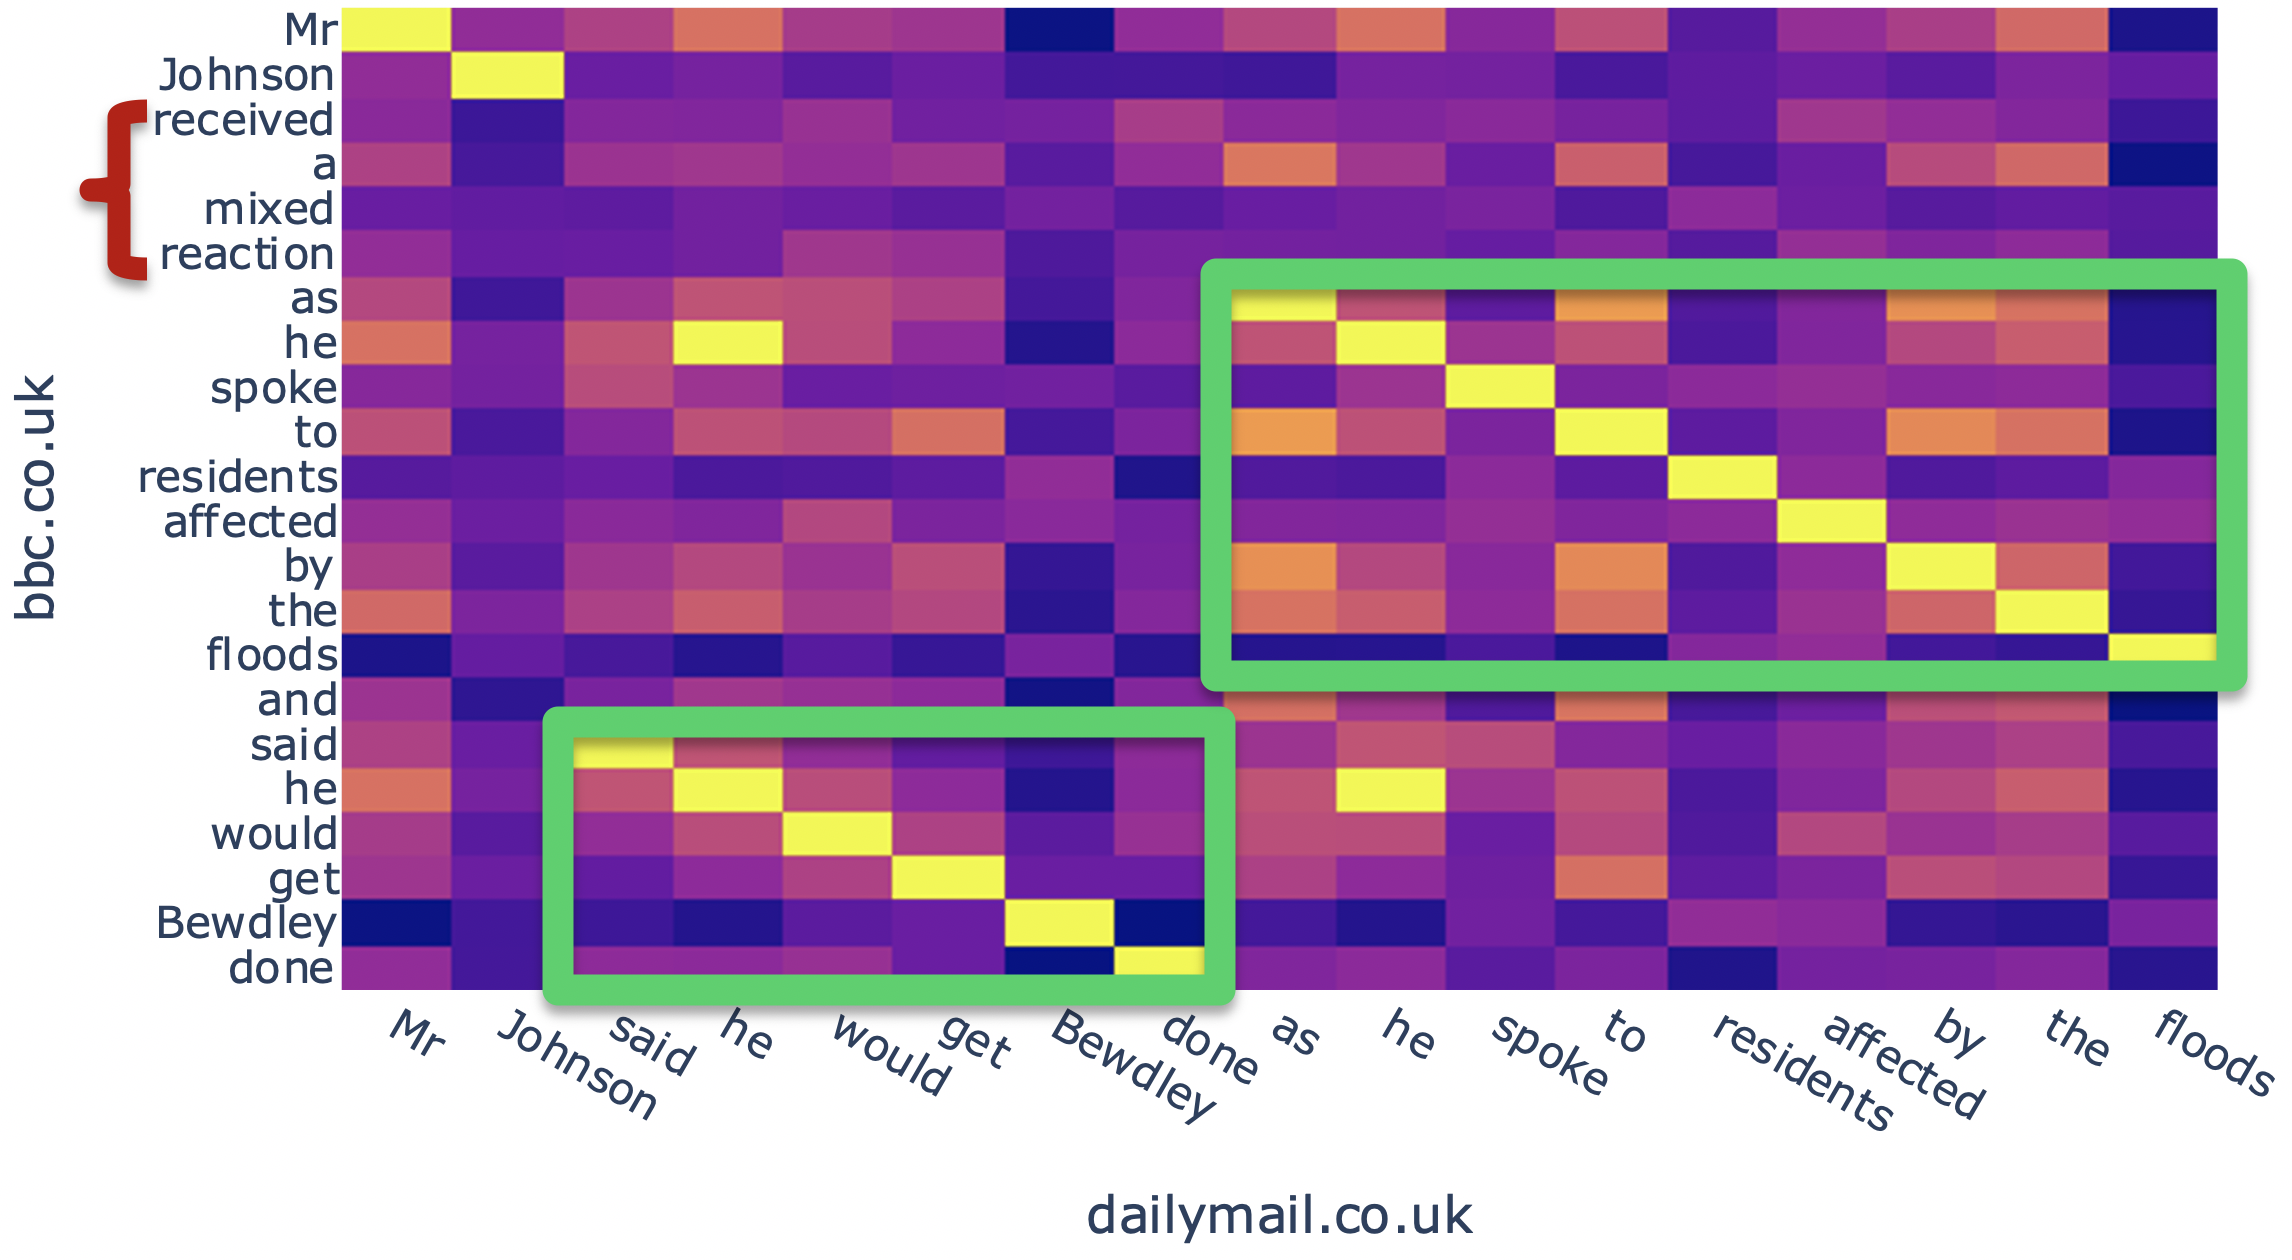
\includegraphics[width=\linewidth]{figures/johnson_flood.png}
    \caption{Example where omitting a detail provides a different framing.}
    \label{fig:johnson_flood}
\end{figure}

% example that needs cross-article analysis
If we take the example of Figure~\ref{fig:johnson_flood}, we take two sentences coming from two different news outlets (on the vertical axis from BBC\footnote{\url{https://www.bbc.co.uk/news/uk-england-hereford-worcester-51791346}} while on the horizontal from Daily Mail\footnote{\url{https://www.dailymail.co.uk/news/article-8088805/Britons-facing-heavy-downpours-four-inches-rain-50mph-winds-set-batter-UK.html}}) and compare the words they contain by using a similarity metric~\cite{cer2018universal}.
From this figure we can see that in the green boxes we have information reported from both sources, while in the red curly brace we have a detail that has been reported only by the BBC.
This specific detail, describing a ``mixed reaction'', gets omitted from the sentence from Daily Mail that is known to be right-leaning\footnote{\url{https://mediabiasfactcheck.com/daily-mail/}}.
% Daily Mail: "While many locals greeted him warmly, he also faced heckles of 'traitor' as he viewed flood barriers - and one person told him to 'do your f***ing job' as he posed with teenagers for a selfie on a bridge in the town."

% limitation of current framing
This example present one specific manifestation of framing that current techniques do not focus on detecting, that is the selection of details.
And the main reason is that such techniques requires a method that goes beyond the analysis of one single article at a time.
We cannot know when something has been omitted if we don't have or a ground truth or different stories to corroborate with, using the richness of information available from multiple points of view.
% RQ1.1 lift
There are facets of framing that have not been tackled by automated approaches because they cannot be pointed out by considering a single article, and we need to investigate which ones we can define more rigorously and how important they are.

% acknowledge existing works on framing differences, but manual and not annotated
% Manual framing difference approaches
There exist some efforts in this joint area, that try to provide multiple points of view of the same events by considering sources that come from different political leanings.
For example, AllSides\footnote{\url{https://www.allsides.com/story/admin}} is a platform that collects articles from different news sources providing a hand-curated set of stories where articles with different political bias are put together, with also a brief textual introduction of the framing differences.

\begin{figure}[!htb]
    \centering
    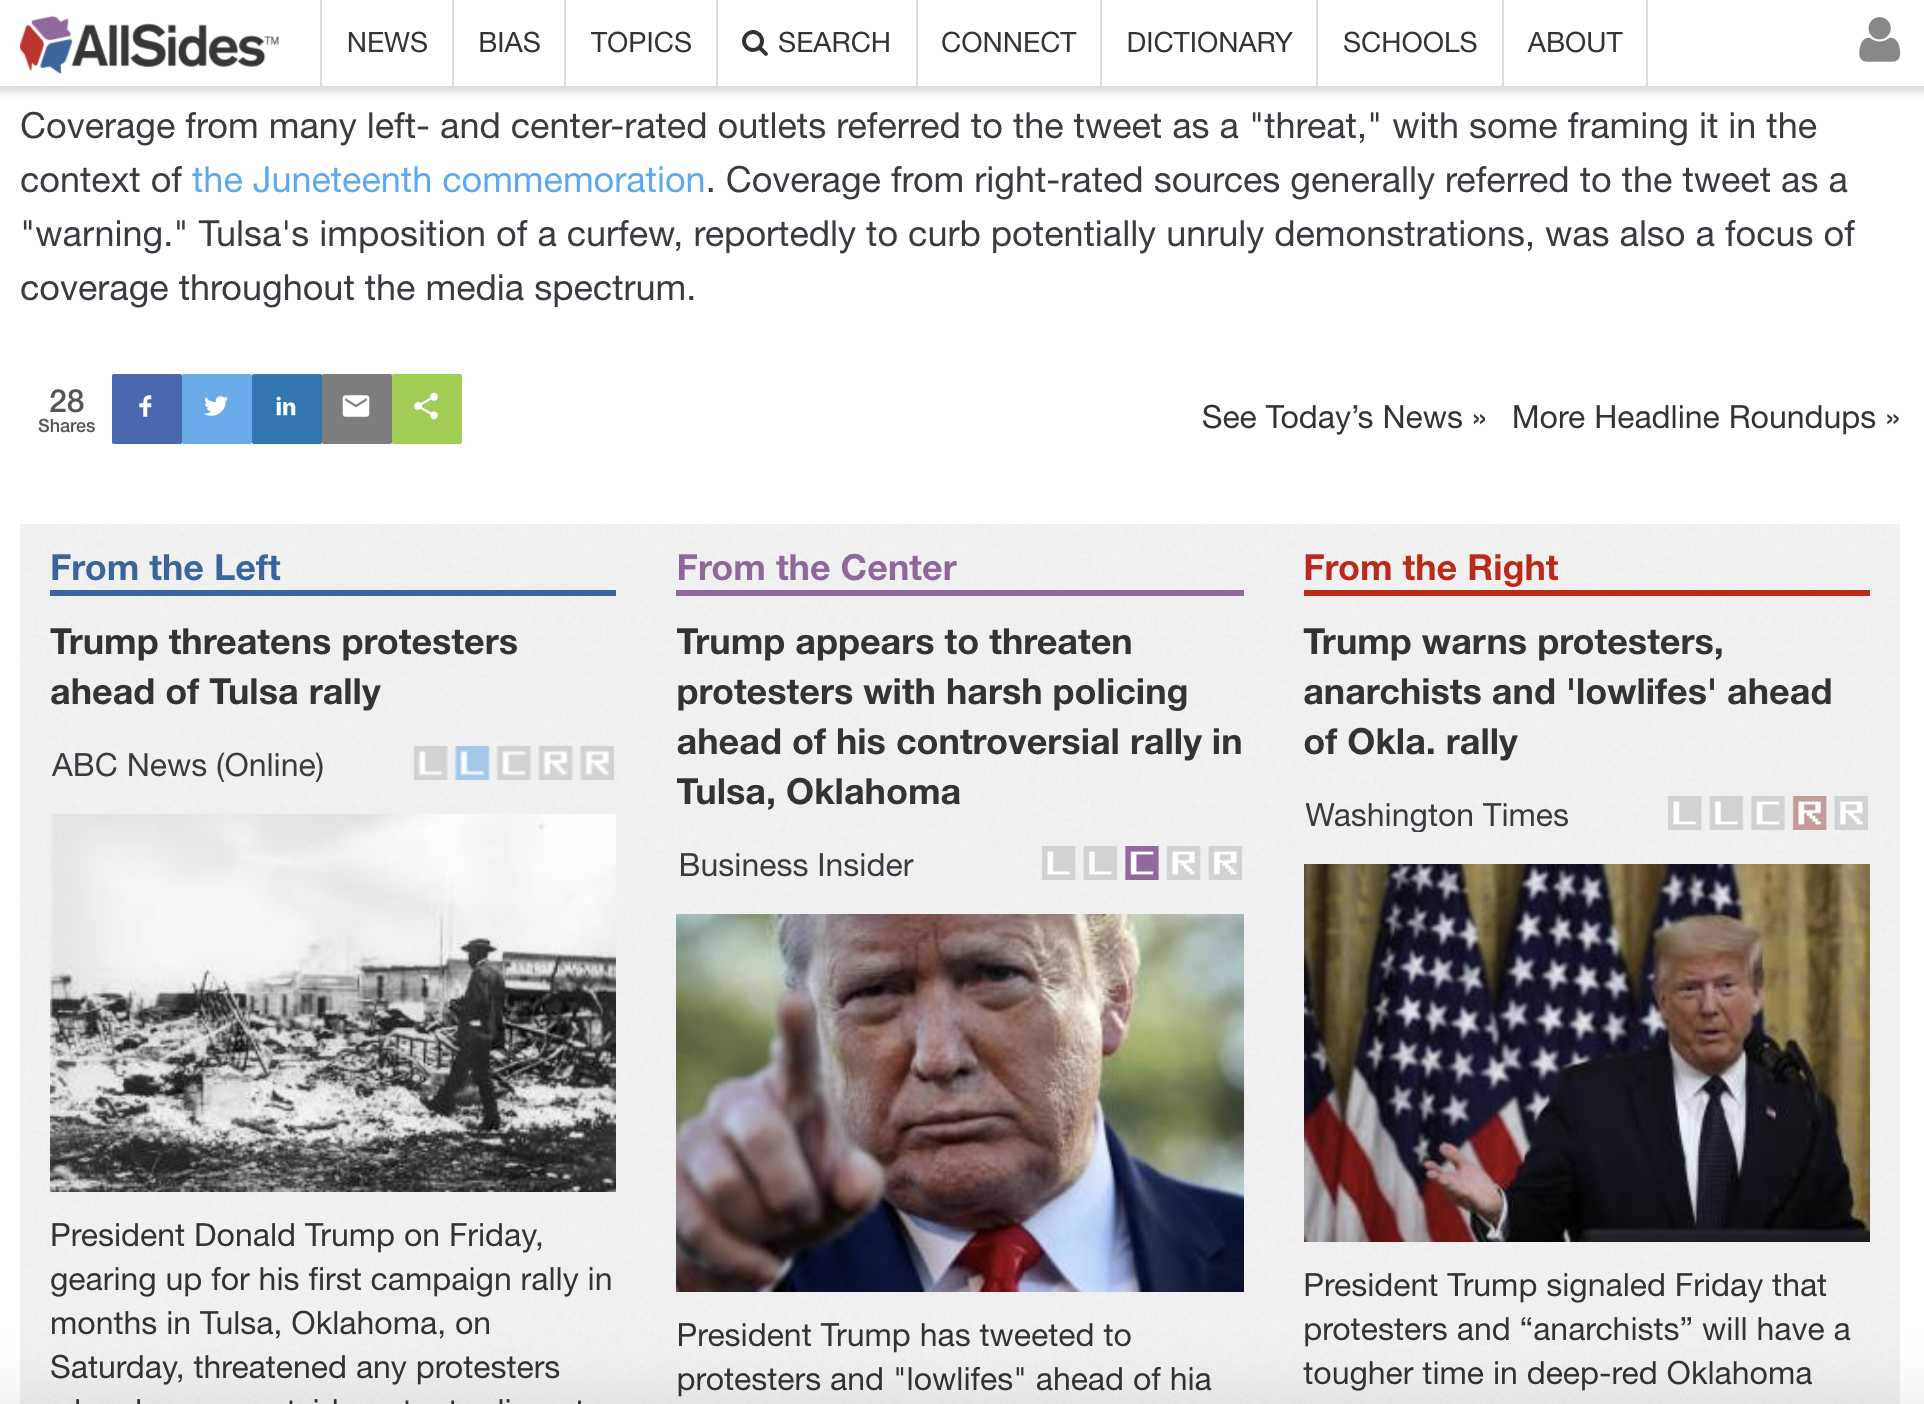
\includegraphics[width=\linewidth]{figures/allsides.png}
    \caption{Example of analysis from AllSides: \url{https://www.allsides.com/story/trump-tweets-about-protesters-ahead-saturday-tulsa-rally}}
    \label{fig:allsides}
\end{figure}

In Figure~\ref{fig:allsides} we can see an example that is displaying how a source from the left, one from the center and one from the right frame differently Trump tweeting about his upcoming rally in Tulsa.
% - which signals
Sources from the left use the term ``threat'' while sources from the right use ``warning'', which can be seen in the specific words used in the headlines.
This \emph{selection of terms} gives a specific framing which can be seen as an emphasis from the left on the strength of the tweet versus an attenuation of the right, plus the centre is instead keeping in an intermediate position.
But if we look at the articles, this term is not the only difference. The sources from the left give more space to the narrative about Juneteenth\footnote{\url{https://en.wikipedia.org/wiki/Juneteenth}} and the past history of the city, which emerges also in the image of the article from ABC News.
We need to have a more precise definition of what constitutes framing and how it manifests in the articles.
% - how could we detect
% - bias vs framing?


% limitations:
% Only US, handmade (lift RQ1.2)
Considering AllSides, its main limitations are due to the fact that the analysis is handmade and therefore they publish just a few stories per week and only focusing on the US.
With this work we want to provide a similar analysis but powered by an automated method, which will need to rely on existing works of framing analysis and document similarities.


% - break your bubble and similar (Blue Feed, Red Feed): feed populated with news from different sides. But not specific on a certain event.

% lack of automated framing difference analysis
We argue that by the integration of these two fields, a deeper analysis of framing can be achieved, with the goal to understand better how, from the same event, multiple stories are generated.

% Framing analysis, being limited to single-article analysis, cannot analyse specific framing manifestations that have been described in theoretical works: for example selecting or omitting details. This is the area that we want to tackle.

% just left-right political leaning is considered (lift RQ2.1)
With respect to AllSides or other tools (Blue Feed, Red Feed\footnote{\url{https://graphics.wsj.com/blue-feed-red-feed/}}) that just focus on the left/right political bias (mainly from US with liberal/conservative), we want to conduct an analysis that compares several characteristics of the news outlets, such as the newsgroup they belong to, or how they are rated by multiple news rating organisations (factuality, bias), or their ideology in general.

% \todo{buildup floor to subquestions}


% 1.1 Need for signals

% 1.2 Need for baseline

% 2.1 Correlation source bias/features

% 2.2 Temporal chains
\todo{RQ2.2???}





% \section{Early draft - remove and merge}

% For this reason, in this chapter we first focus on works that analyse how documents are talking about the same details, using language representations, clustering and seeing which details are narrated by different sources.
% The objective of this first group is to extract the common ground between different stories and highlight the pieces that are uniquely changed, added or removed by individual sources.

% Then we present works that characterise documents with linguistic features that we aim to use for the second phase, that is \emph{understanding} the framing that the choices of the authors use. For this reason, we analyse a set of features that have appeared in similar works.





% \section{Linguistic features}

% While the first group of works focuses on finding similar articles and highlighting parts that are similar or different, here we present a set of linguistic features that can be very useful in order to characterise the peculiarities. These works are usually independent from our goal, and are applied in a wide variety of tasks.

% \subsection{Natural Language Parsing}

% % grammar, POS, dependencies, entity extraction and linking
% First of all, we have a set of features that comes to represent the structure of sentences. It is the world of parsers, that are able to tokenise, find Part Of Speech and create Dependency Trees.

% The progress of this research is quite advanced, and there are plenties of tools available off-the-shelf (e.g. Stanford NLP, SpaCy, ...) that achieve good performances (TODO?)

% entities (WARNING: avoid duplicate with 2.1.1. Language Representation)



% \subsection{Bias and Framing}



% \section{Gaps}

% TODO: underline lack of approaches and studies that accomplish the task automatically.

% All these features have been used in previous research, but as mentioned above, they are mainly applied to single-article analysis. Extending this kind of analysis by taking into consideration the relationships both at the article level and the sentence level would bring a big contribution by providing contrastive signals that would not come up otherwise. 

% \label{sec:related}

In this section, we provide an overview of previous studies in two areas of research. First, the investigation on relationships between news articles which aims to find documents that cover the same information. Second, the detection of narrative linguistic signals, which investigates and characterises several aspects of structure, framing, and subjectivity.
For both of them, we gather a set of techniques that enable our approach described in the next Section~\ref{sec:framework}.
%can be used to characterise the components(sentences/paragraphs) of the articles.
%can help us characterise the narrative comparison analysis.
%Starting from approaches that link together articles and parts of articles together that cover the same information, we see how we can enrich and characterise the participating nodes (articles and sentences) with signals from narrative, framing and subjectivity analysis.

%\todo[color=yellow]{add a sentence here to remark that we just observed works on the two areas, separated and not joint?}

\begin{comment}
    % 2: Main limitations of existing works
    But there are different limitations of what is available.
    For example, the approach proposed by~\cite{bountouridis2018explaining} finds and links similar articles and similar sentences (POI) in them, but mainly focuses on finding indications of corroborated information or omitted information.
    Their work does not investigate the differences between the linked pieces, accounting for subtle modifications and their exploitation to provide bias / subjectivity (framing / word choices).
    Another recent work~\cite{zahid2019towards} instead is just focusing on a single article narrative analysis, without linking and comparing it to other news articles.
    \todo[color=yellow]{move this paragraph to related work, just leave a sentence here}
\end{comment}

\subsection{Relationships between news articles}

% Definition of relationship
There are different possible types of relationships between news articles, such as similarity (covering the same information), referencing (one is citing another one), and temporal proximity. They can be performed at the document level (e.g., the whole article is similar to another one) or at the sentence level (e.g., the same sentence is corroborated by a sentence in another article~\cite{bountouridis2018explaining}) or even at the paragraph level.
Since we are interested in finding articles discussing the same information, we focus on similarity relationships.
% \begin{added}
Other relationships could add interesting features, such as the order of publication which would help to identify which of the articles might have taken inspiration from the other. For the time being, we focus on studying and understanding the role of similarity.
% \end{added}
%In this direction it is very important to keep exposed to multiple perspectives~\cite{flaxman2016filter}, thanks to news aggregators, that provide articles on the same events from multiple sources (e.g. Google Headlines\footnote{\url{https://news.google.com/}}) or approaches that analyse the corroboration and omission between news articles~\cite{bountouridis2018explaining}. 

% Article-level relationships
At the article-level, there is a wide variety of work that investigates article clustering, and the methods mostly used are Latent Dirichlet Allocation (LDA) or document embedding.
% News aggregators and LDA topic: can provide article-level aggregation
LDA~\cite{blei2003latent} is the most used technique for topic modelling, as it allows the discovery of topics and to group articles accordingly using word distributions.
% similarity measures
Another technique for grouping articles together is to compute a similarity measure (e.g., cosine similarity) between numeric representations of the documents (TF-IDF~\cite{jones1972statistical} or Language Models~\cite{devlin2018bert,cer2018universal,yang2019xlnet}).
% \begin{added}
We plan to study these models in order to select the one that can efficiently discriminate articles that talk about the same events, even if they use different linguistics, from articles that may use the same subset of words but talk about different events. 
% \end{added}
%In this direction, there are several techniques, such as TF-IDF~\cite{jones1972statistical} or using representations coming from Language Models~\cite{devlin2018bert,cer2018universal,yang2019xlnet}.
% recent advances on similarity and document embedding
%But with the recent explosion of Deep Learning representation there emerged many of Language Model tools that can provide document representation, like BERT~\cite{TODO}, XLnet~\cite{TODO}, or even more oriented towards the similarity task: Universal Sentence Encoder~\cite{TODO}.\todo[color=yellow]{too many details on possible features for similarity?}
% And all these models can be used directly without the need to train, thanks to pretrained models that perform already well out-of-the-box.


% Topic Detection and Tracking steps
% 0. flat clusters: TDT before 2003. Simple LDA clustering methods
% 1. hierarchical topics: TDT 2003 (hierarchy of topic --> event --> story)
% 2. dependencies: 2004 Napallati~\cite{nallapati2004event}. They introduce edges with two possible reasons: causality or only temporal ordering.

% News event structure evolution (keep short)
% Instead in the direction of the structure of news event, we have a succession of works that went more in details than just creating groups / flat clusters generated by LDA.
% First of all \emph{hierarchical} topic modelling~\cite{allan2003flexible} that defined a set of levels (from the broad concept of topic, to the narrow event that belongs to the topic, and then a specific story/anecdote).
% And then moved to study the dependencies between events~\cite{nallapati2004event} with causality and temporal ordering.
% This recently brought to approaches that are able to find the events belonging to a topic and link them creating a Event Evolution Graph~\cite{yang2009discovering,ansah2019graph} that can be visualised to give an idea of the dependency between the events detected.
%\todo[color=yellow]{The removed paragraph was about events hierarchy and dependency}
% ~\cite{ansah2019graph} that is able to generate a visual story timeline summarisation, connecting the main events; Event Maps~\cite{yang2009discovering}
% Or works that focus on the illustrative side and use the extracted story timeline summarisation~\cite{ansah2019graph}.

% Furthermore, \cite{cai2019temporal} also presents event maps (original baseline~\cite{yang2009discovering}). With also importance score on the nodes and edges. The event relationships can be temporal, content dependence and event dependence.


% Corroboration, external confirmation / denial: computation and visualisation. \cite{bountouridis2018explaining}
Furthermore, there are works that not only link the articles at a document level, but also investigate in more detail the connections between sentences.
In one recent work~\cite{bountouridis2018explaining}, groups of similar articles are found, then broken down to pieces of information and analysed to find if these details are \emph{corroborated} (occurring in multiple documents) or \emph{omitted} (occurring in other documents of the same group, but not the current one). 
%is good for getting relationships between paragraphs and documents. Corroboration and omission
% \begin{added}
We aim to use this idea of applying similarity to both article-level and sentence-level, extending it even to the word-level. By doing so,
not only we might be able to recognise which sentences appear in multiple documents (with different degrees of similarity) but also we would be able to identify the specific words that have been changed.
%, on one side we will be able to keep the information of similarity and on the other side we will bring into view the differences of the articles (sentences) and sentences (words).
% \end{added}

% \removed{When looking at the results of such approaches, it is often left to the reader to evaluate and compare the linked information pieces.}
% \begin{added}
However, this set of approaches are limited to bringing to the attention of the reader the linked information pieces with a measure of similarity, without characterising the differences. The reader would then need to evaluate the differences in the role of the sentence, the framing that it implies and how it compares with other sentences in terms of subjectivity.
Different documents may express the same set of details, but give them a different role (reporting an action, commenting, contextualising, doing a digression, identifying causes and consequences) and use different words that are semantically similar but may imply a different framing perspective.
For this reason, the next subsection presents a set of narrative linguistic signals that could provide us with the missing features.
% \end{added}
% \removed{A sentence can have different roles in a document (reporting an action, commenting, contextualising, doing a digression) and hence it is important to extract and present these features.
% Furthermore, even if the information is reported in similar ways in different articles, they could be using specific choices of words to provide a different framing.}
%We see these difference, as signals, in the following subsection.

%The only cross-document narrative analysis found~\cite{reiter2014nlp} (structural similarity, using FrameNet)~\todo[color=yellow]{move this sentence in the proper position}

% Some directions used by document comparison:
% - fact-checking: \cite{karadzhov2017fully} automatic fact-checking by comparing news article
% - perspectrum: \cite{chen2019seeing} presents PERSPECTRUM, comparing stance and perspectives for a claim.
% - break your bubble or similar news aggregators (Balancer, Blue Feed Red Feed, Burst your bubble, Escape your bubble, Read Across the Isle, OneSub, Nuzzera)

\subsection{Narrative linguistic signals}
% \subsection{The many faces of \sout{biases}: Narrative, framing and subjectivity/bias signals}
%\todo{define somewhere the term \emph{narrative linguistic signal}}
% The term mainly comes from http://ceur-ws.org/Vol-2342/paper9.pdf where they use "linguistic devices". "Devices" was then substituted with "signals". About "linguistic signal", there are many works that use it https://www.aaai.org/ocs/index.php/ICWSM/ICWSM16/paper/download/13112/12731 https://www.shanjiang.me/publications/cscw18a_paper.pdf
% It's in general some words that signal something (structure / framing / subjectivity). And "narrative" because it encloses structure, framing and subjectivity. 

There is much research on exposing the narrative using linguistic signals~\cite{zahid2019towards}, with specific words that indicate the \emph{structural role}, \emph{framing} and \emph{subjectivity} of the part of text they belong to.
%There is a wide literature of work that wants to expose the narrative using linguistic signals, with specific words that indicate the \emph{structural role}, \emph{framing} and \emph{subjectivity} of the part of text they belong to.
One limitation is that most of such works are applied to single articles, with little comparison between them.
%\todo[color=yellow]{put this at the end of subsection, to bridge what we want to do?}

% news schema structure
On one hand, some research considers the \emph{structural role} of a sentence in the document (e.g., is it providing some background, the main event, an evaluation).
Different structural roles have been defined in the literature, such as 
%Different works define sets of structural roles: 
news schema~\cite{bell1991language}, which identifies hierarchical categories (e.g., action, reaction, consequence, context, history), narrative structure~\cite{bell2005news} (e.g., abstract, orientation, evaluation, complication, resolution), or linguistic signals~\cite{zahid2019towards,marcu2000theory}. 
%One recent study~\cite{zahid2019towards} proposed linguistic signals to be able to recognise the structural role.
%With such characterisations, we would be able to add to the sentence-level similarity links also their role in the different articles, to understand how their structure differs.
Such signals could be used to identify the differences between similar sentences with regards to their structural roles in the articles. 
% And this is an important feature because time structure and story structure are usually different~\cite{bell2005news}.

% framing
On the other hand, there is much literature on \emph{framing}, defined
as how a certain story is presented to shape mass opinion~\cite{goffman1974frame}, the addition to the underlying facts that reflects the sociocultural context
%(cultural, political, ...)
and acts as an underlying force to persuade the reader.
% Semantic frames~\cite{fillmore2006frame}
% News Media Frames~\cite{boydstun2014tracking} developed a schema of 15 cross-cutting framing dimensions, such as economics, morality, and politics, and
% dataset of human annotations~\cite{card2015media}
The work by~\cite{gamson1989media} describes a set of \emph{framing packages}, made of \emph{framing devices} (e.g., word choice, metaphors, catchphrases, 
%exemplars, depictions, descriptions, 
use of contrast, quantification) and \emph{reasoning devices} (e.g., problem definition, cause, consequence, solution, action%, moral evaluation
).
Additionally, the Frame Semantics Theory~\cite{fillmore2006frame} can be used to recognise lexical units of known frames.
By extracting these linguistic signals, we could represent the framing behind a certain piece of text, and there exist different approaches to extract the listed features~\cite{mandal2017overview,gao2018neural,asghar2016automatic,swayamdipta:17}.

In addition to these two characterisations, we can add other signals derived from studies on \emph{subjectivity}.
% and sentiment intensity.
% https://www.niemanlab.org/2019/05/u-s-journalism-really-has-become-more-subjective-and-personal-at-least-some-of-it/ "a blurring of the line between opinion and fact."
As found by recent research, in contemporary journalism the line between opinion and facts is blurring more and more~\cite{blake2019news}. For this reason, having signals of subjectivity on the document and paragraph-level would be very useful~\cite{liu2010sentiment}.
%Furthermore, subjectivity is closely related to sentiment, since sentiment analysis is about finding the value of opinion while subjectivity is about distinguishing if the text is having an opinion or just reporting factual events~\cite{liu2010sentiment}.
In this way, each article and each paragraph can be characterised with an indication of subjectivity.

% % subjectivity
% Then there is a wide set of works on \emph{subjectivity}
% Studies on subjectivity are good for adding the feature

% % sentiment intensity
% Hate/sentiment intensity: emotional level

% word choices (are a device of framing/subjectivity/intensity)

% \removed{As noted for the first area, also this research would benefit an integration, since a contrastive analysis can have more signals as the single-article equivalent, as we will see in the next session.}
% \begin{added}
All these features have been used in previous research, but as mentioned above, they are mainly applied to single-article analysis. Extending this kind of analysis by taking into consideration the relationships both at the article level and the sentence level would bring a big contribution by providing contrastive signals that would not come up otherwise. 
% \end{added}